\chapter{Environnement de travail}
\label{chap:environnement_travail}

\section{Introduction}

Ce chapitre présente l'environnement technique retenu pour la conception et la réalisation de la plateforme \textit{EcoRewind}. Il décrit l'architecture logicielle de l'application, les outils et technologies mobilisés, ainsi que l'environnement de développement utilisé. Ces choix répondent aux besoins de la plateforme : sensibilisation au tri des déchets, interaction entre les différents acteurs, suivi des points de collecte et remontée d'informations en temps réel depuis les équipements intelligents.

\section{Architecture logicielle}
\label{sec:architecture_logicielle}

Afin de garantir la modularité, la maintenabilité et l'évolutivité de la solution, \textit{EcoRewind} adopte une architecture client--serveur organisée autour d'une application mobile multiplateforme, d'une API REST et de services de données temps réel. Cette organisation sépare clairement l'interface utilisateur, la logique métier et la persistance des données.

\subsection{Description de l'architecture}

L'application cliente, développée avec Flutter, constitue le point d'accès des différents profils : citoyen, éducateur, collecteur, gestionnaire de point, administrateur et super-administrateur. Elle fournit les interfaces de consultation, de sensibilisation, de gestion des collectes, de scan des QR codes et de suivi des récompenses.

La couche métier est assurée par une API REST développée avec FastAPI et Python. Elle centralise les règles de gestion, l'authentification, le contrôle des droits selon les rôles, la validation des opérations et les échanges avec les services externes. L'API est structurée en modules fonctionnels, notamment pour les utilisateurs, les publications communautaires, les points de collecte, les quiz, les notifications, les groupes, les réunions, l'analytique et l'administration.

Les données transactionnelles sont stockées dans PostgreSQL à travers SQLAlchemy et des migrations Alembic. En environnement de développement, SQLite peut être employé comme solution locale de secours. Firebase complète cette persistance pour les données nécessitant une synchronisation immédiate, telles que les scores, l'état des poubelles intelligentes, certaines statistiques administratives et les notifications.

Les équipements intelligents communiquent avec la plateforme à travers les services backend et Firebase. Le scan d'un QR code permet notamment d'identifier le citoyen et le bac concerné, de vérifier les autorisations, d'enregistrer l'opération et de mettre à jour le score. Cette séparation des responsabilités facilite l'évolution indépendante de chaque composant.

\begin{figure}[H]
    \centering
    \frame{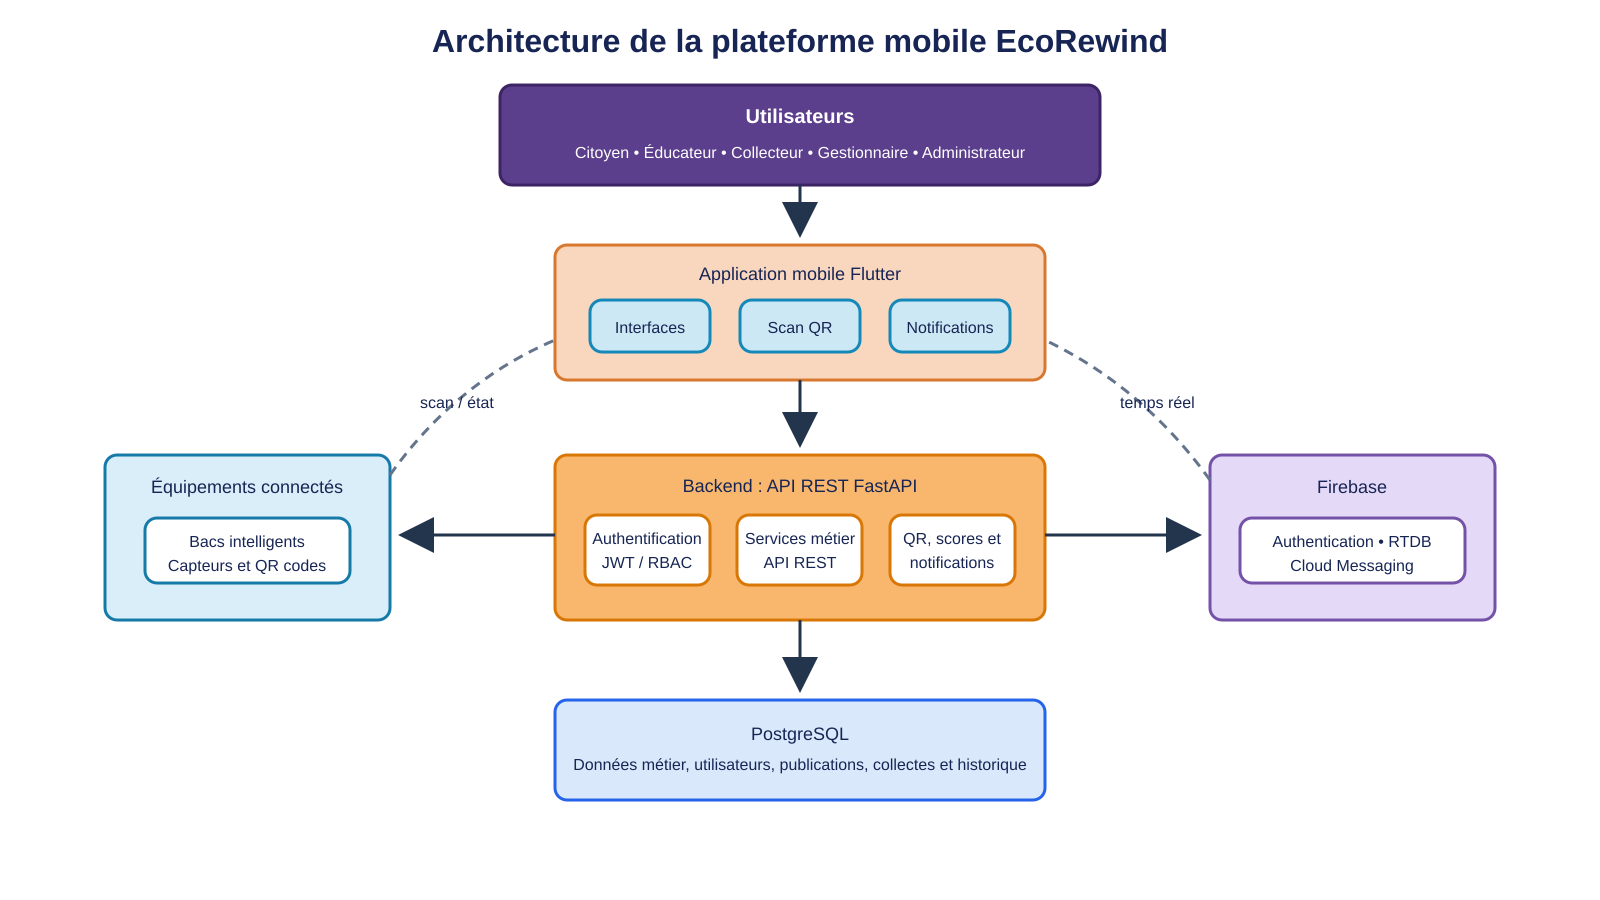
\includegraphics[width=0.90\textwidth]{image/architecture_ecorewind.png}}
    \caption{Représentation générale de l'architecture logicielle d'EcoRewind}
    \label{fig:architecture_ecorewind}
\end{figure}

\subsection{Avantages de l'architecture retenue}

L'architecture de \textit{EcoRewind} présente plusieurs avantages :
\begin{itemize}
    \item \textbf{Séparation des responsabilités :} Flutter prend en charge l'expérience utilisateur, FastAPI porte les règles métier et PostgreSQL assure la persistance transactionnelle. Cette répartition simplifie la compréhension et la maintenance du système.
    \item \textbf{Accès multiplateforme :} grâce à Flutter, une même base de code permet de cibler les environnements mobiles et web, tout en conservant une interface cohérente pour les utilisateurs.
    \item \textbf{Évolutivité fonctionnelle :} les routeurs FastAPI sont organisés par domaine métier. De nouvelles fonctionnalités peuvent ainsi être ajoutées sans remettre en cause l'ensemble de l'application.
    \item \textbf{Temps réel :} Firebase Realtime Database permet de diffuser rapidement l'état des bacs, les scores et les indicateurs administratifs vers les clients autorisés.
    \item \textbf{Sécurité :} l'API s'appuie sur des jetons JWT, les contrôles d'accès par rôle et les règles de sécurité Firebase. Les opérations sensibles restent contrôlées par le backend.
    \item \textbf{Fiabilité des données :} PostgreSQL et les migrations Alembic permettent de conserver un schéma de données versionné et cohérent au fil des évolutions du projet.
\end{itemize}

\subsection{Architecture technique}

La figure \ref{fig:architecture_technique_ecorewind} détaille les principaux flux techniques de la solution. L'utilisateur interagit avec l'application Flutter, qui appelle l'API FastAPI au moyen de requêtes HTTP sécurisées. L'API applique la logique métier, accède à PostgreSQL pour les données persistantes et communique avec Firebase au moyen du SDK d'administration pour les informations temps réel.

Firebase Authentication permet au client de s'authentifier auprès des services Firebase lorsque cela est nécessaire. Firebase Cloud Messaging est utilisé pour les notifications push, tandis que Firebase Realtime Database met à disposition des flux de lecture temps réel. Les clients Flutter restent en lecture seule sur les nœuds sensibles ; les écritures sont réalisées par le backend, ce qui renforce le contrôle des données. Les fichiers téléversés sont servis par l'API depuis l'espace dédié aux téléversements.

\begin{figure}[H]
    \centering
    \frame{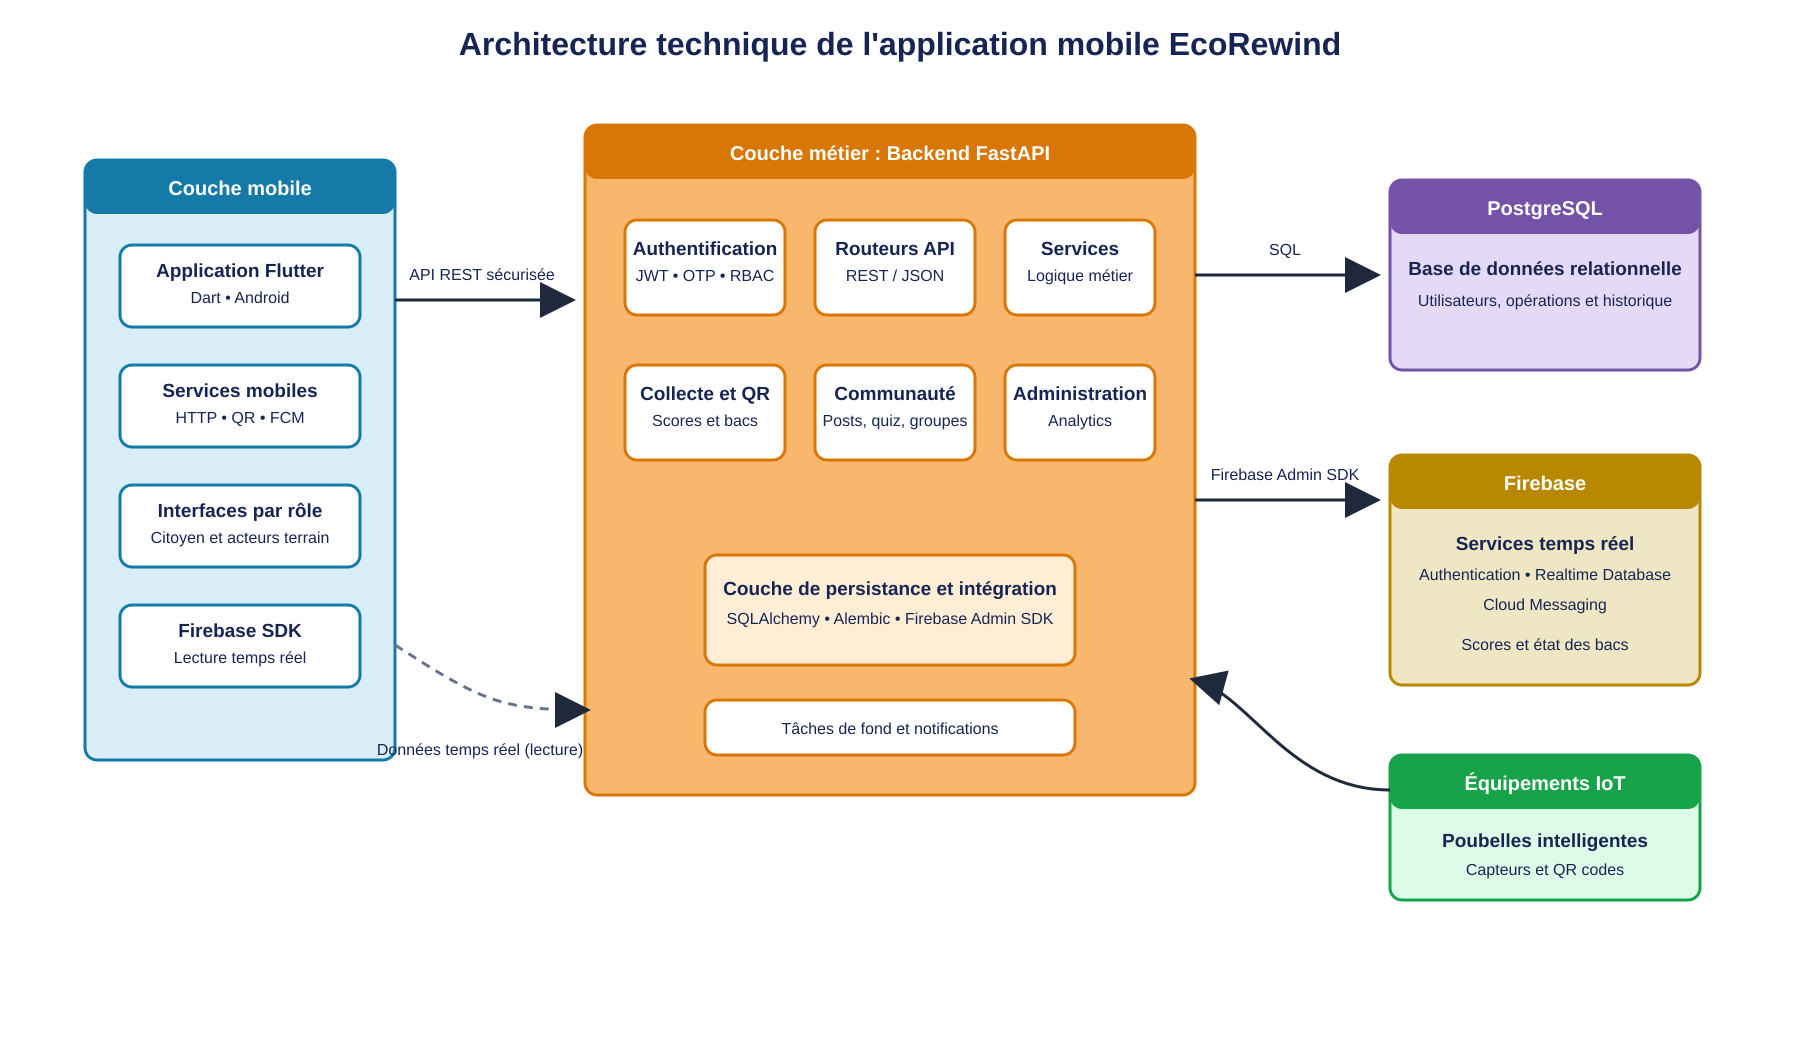
\includegraphics[width=0.95\textwidth]{image/architecture_technique_ecorewind.png}}
    \caption{Architecture technique de la plateforme EcoRewind}
    \label{fig:architecture_technique_ecorewind}
\end{figure}

\section{Outils et technologies}
\label{sec:outils_technologies}

Le choix des technologies a été orienté par la compatibilité multiplateforme, la rapidité de développement, la sécurité des accès et la capacité à gérer des données environnementales en temps réel.

\subsection{Développement frontend : Flutter et Dart}

Flutter est le framework utilisé pour développer l'application cliente, tandis que Dart est le langage de programmation associé. Cette combinaison permet de produire une application multiplateforme à partir d'une base de code unique. Elle est particulièrement adaptée à \textit{EcoRewind}, car les citoyens et les acteurs opérationnels doivent pouvoir consulter les informations et interagir avec la plateforme depuis différents supports.

L'application Flutter regroupe notamment les interfaces de géolocalisation et de consultation des points de collecte, de scan QR, de suivi des scores, de quiz, de publications communautaires, de messagerie, de notifications et de tableaux de bord adaptés aux rôles.

\subsection{Développement backend : Python et FastAPI}

Le backend est développé en Python avec le framework FastAPI. FastAPI facilite la création d'API REST performantes, structurées et documentées. Il est utilisé pour exposer les services consommés par l'application Flutter, valider les données, gérer les droits d'accès et centraliser les traitements métier.

L'API \textit{EcoRewind} est organisée en routeurs spécialisés, tels que l'authentification, la gestion des utilisateurs, les publications, les points de collecte, les quiz, les groupes, les réunions, l'analytique et les fonctions d'administration. Cette structuration améliore la lisibilité du code et permet de faire évoluer les modules de manière maîtrisée.

\subsection{Base de données : PostgreSQL, SQLAlchemy et Alembic}

PostgreSQL est utilisé comme système de gestion de base de données relationnelle pour l'environnement de production. Il stocke les informations structurées de la plateforme, dont les comptes, les rôles, les points de collecte, les publications, les interventions et les données de suivi.

SQLAlchemy assure la couche de persistance entre les modèles Python et la base de données. Alembic permet de versionner et d'appliquer les migrations du schéma de données. Cette approche garantit une évolution contrôlée de la base au cours des itérations. SQLite est également disponible pour les essais locaux en développement, sans être destiné à un déploiement de production.

\subsection{Services Firebase}

Firebase est intégré pour les besoins de synchronisation et de communication en temps réel :
\begin{itemize}
    \item \textbf{Firebase Authentication} prend en charge l'authentification auprès de l'écosystème Firebase à partir de jetons générés par le backend ;
    \item \textbf{Firebase Realtime Database} diffuse en lecture les scores des citoyens, l'état des bacs intelligents, les profils nécessaires aux équipements et des statistiques administratives ;
    \item \textbf{Firebase Cloud Messaging} permet l'envoi de notifications push vers les appareils mobiles.
\end{itemize}

Cette intégration améliore la réactivité de la plateforme, notamment lors de l'évolution de l'état d'un bac ou de l'attribution de points après un scan.

\subsection{Sécurité et authentification}

La sécurité des échanges repose sur des jetons JWT émis par le backend. Chaque requête protégée est vérifiée avant l'accès aux ressources. Le contrôle d'accès fondé sur les rôles limite les actions disponibles selon le profil connecté. Les mots de passe sont stockés sous forme hachée et des mécanismes complémentaires, tels que les codes OTP et l'authentification multifacteur, renforcent la protection des comptes lorsque cela est requis.

Les règles Firebase interdisent les écritures directes du client sur les données sensibles. Le backend, au moyen du SDK Firebase Admin, reste l'intermédiaire responsable des mises à jour critiques.

\subsection{Outils de développement et de collaboration}

Les principaux outils employés pour la réalisation et la validation de la solution sont les suivants :
\begin{itemize}
    \item \textbf{Visual Studio Code :} éditeur de code utilisé pour le développement Flutter, Python et les fichiers de configuration ;
    \item \textbf{Android Studio et les outils Flutter :} utilisés pour l'émulation, le débogage et les tests de l'application Android ;
    \item \textbf{Postman :} utilisé pour tester les points d'entrée de l'API REST, vérifier les réponses et valider les scénarios d'authentification ;
    \item \textbf{Git et GitHub :} utilisés pour le versionnement du code source, la sauvegarde des évolutions et la collaboration ;
    \item \textbf{Draw.io :} utilisé pour concevoir les diagrammes d'architecture, de flux et de modélisation présentés dans le rapport ;
    \item \textbf{Firebase Console :} utilisée pour administrer la configuration Firebase, les données temps réel et les services de notification.
\end{itemize}

\section{Environnement de développement}
\label{sec:environnement_developpement}

L'environnement de développement réunit les outils nécessaires à la construction, à l'exécution et au test des différentes couches de \textit{EcoRewind}. Le client Flutter est exécuté sur un émulateur Android, un appareil physique ou un navigateur web. Le serveur FastAPI est lancé localement afin d'exposer l'API REST, tandis que PostgreSQL est configuré au moyen des variables d'environnement du projet.

Le cycle de développement consiste à implémenter ou ajuster une fonctionnalité côté Flutter et FastAPI, appliquer les migrations de base de données avec Alembic lorsque le schéma évolue, puis tester les services par l'interface Swagger fournie par FastAPI ou avec Postman. Les fonctions nécessitant des données temps réel sont ensuite vérifiées avec Firebase.

\begin{figure}[H]
    \centering
    \frame{\includegraphics[width=0.85\textwidth]{image/environnement_developpement_ecorewind.png}}
    \caption{Environnement de développement et outils utilisés pour EcoRewind}
    \label{fig:environnement_developpement_ecorewind}
\end{figure}

\subsection{Environnement matériel}

Le développement et les tests ont été réalisés sur un ordinateur disposant d'un système d'exploitation compatible avec Flutter, Python, PostgreSQL et les outils de développement associés. Le tableau \ref{tab:environnement_materiel} présente un modèle de description de l'environnement matériel à compléter avec les caractéristiques de la machine utilisée.

\begin{table}[H]
\centering
\renewcommand{\arraystretch}{1.2}
\begin{tabular}{|p{5cm}|p{8cm}|}
\hline
\textbf{Caractéristique} & \textbf{Détail} \\
\hline
Système d'exploitation & À compléter (par exemple : Windows 11) \\
\hline
Processeur & À compléter \\
\hline
Mémoire installée (RAM) & À compléter \\
\hline
Machine utilisée & À compléter \\
\hline
\end{tabular}
\caption{Caractéristiques de l'environnement matériel}
\label{tab:environnement_materiel}
\end{table}

\section{Conclusion}

Ce chapitre a présenté l'environnement de travail de la plateforme \textit{EcoRewind}. L'architecture client--serveur choisie associe Flutter pour l'interface multiplateforme, FastAPI pour les services métier, PostgreSQL pour la persistance relationnelle et Firebase pour les données et notifications en temps réel.

Ces choix permettent de répondre aux besoins fonctionnels de la plateforme tout en préservant la séparation des responsabilités, la sécurité des accès et la capacité d'évolution. L'environnement de développement et les outils de test retenus constituent ainsi une base cohérente pour poursuivre la réalisation, la validation et le déploiement des différents modules d'EcoRewind.
